
\documentclass{report} 
\usepackage{graphics} 
\usepackage{graphicx} 
\usepackage{mathtools} 
\usepackage{amsmath} 
\usepackage{amssymb} 
\usepackage[margin = 1in]{geometry}

\graphicspath{
	{/Users/astrobeard/Work/Research/VICErepos/VICE/migration/figures/}
}

\begin{document} 

\begin{figure*} 
\centering 
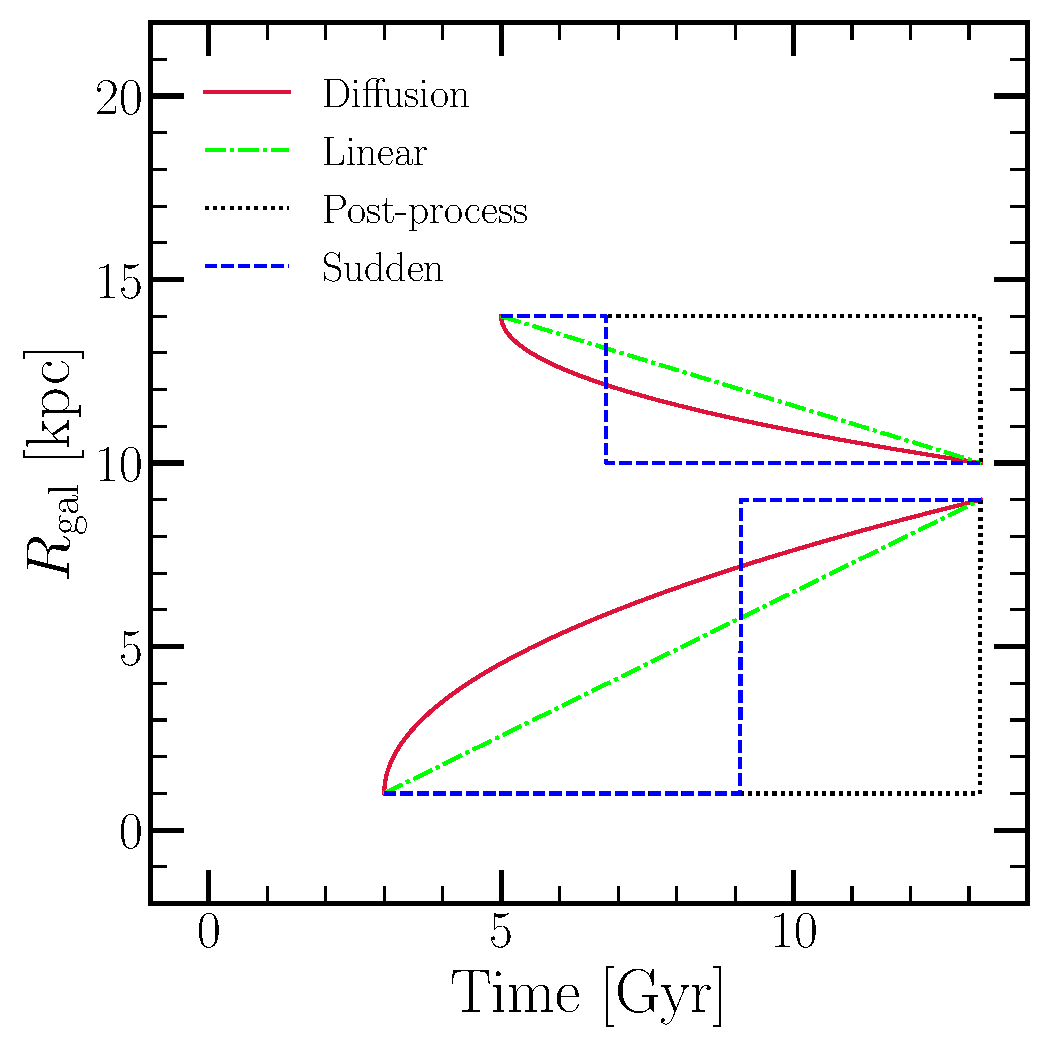
\includegraphics[scale = 0.5]{migration.pdf} 
\caption{A diagram illustrating our migration schema: diffusion (crimson, 
solid), linear (lime, dot-dashed), post-process (black, dotted), and sudden 
(blue, dashed), for three sets of initial and final radii and birth times. 
These values are pseudorandom numbers drawn from a uniform distribution for 
illustrative purposes. With the initial and final Galactocentric radii of a 
stellar population, its birth time, and one of these assumptions about the 
time-dependence of radial migration, the Galactocentric radius at all times 
is known. } 
\end{figure*} 

\begin{figure} 
\centering 
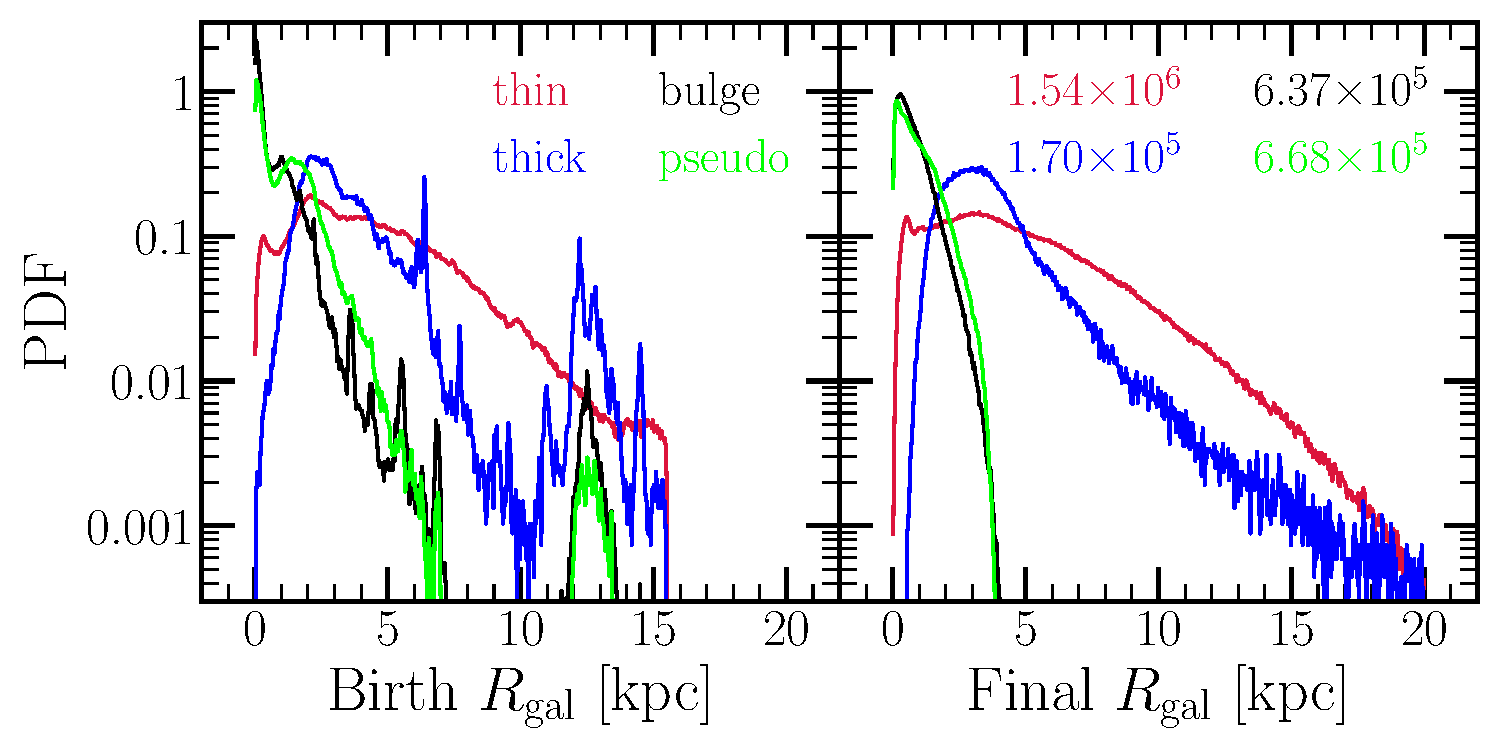
\includegraphics[scale = 0.5]{h277/birth_final_radii_pdfs.pdf} 
\caption{Distributions of~\texttt{h277} star particles in their birth (left) 
and final (right) Galactocentric radii. Distributions are shown for thin 
disk (crimson), thick disk (blue), bulge (black), and pseudobulge (lime) 
populations according to the kinematic decomposition described in~\S~X. 
In the right-hand panel we denote the number of star particles in each 
population according to the same color-coding. } 
\label{fig:h277_birth_final_radii_pdfs} 
\end{figure} 

\begin{figure*} 
\centering 
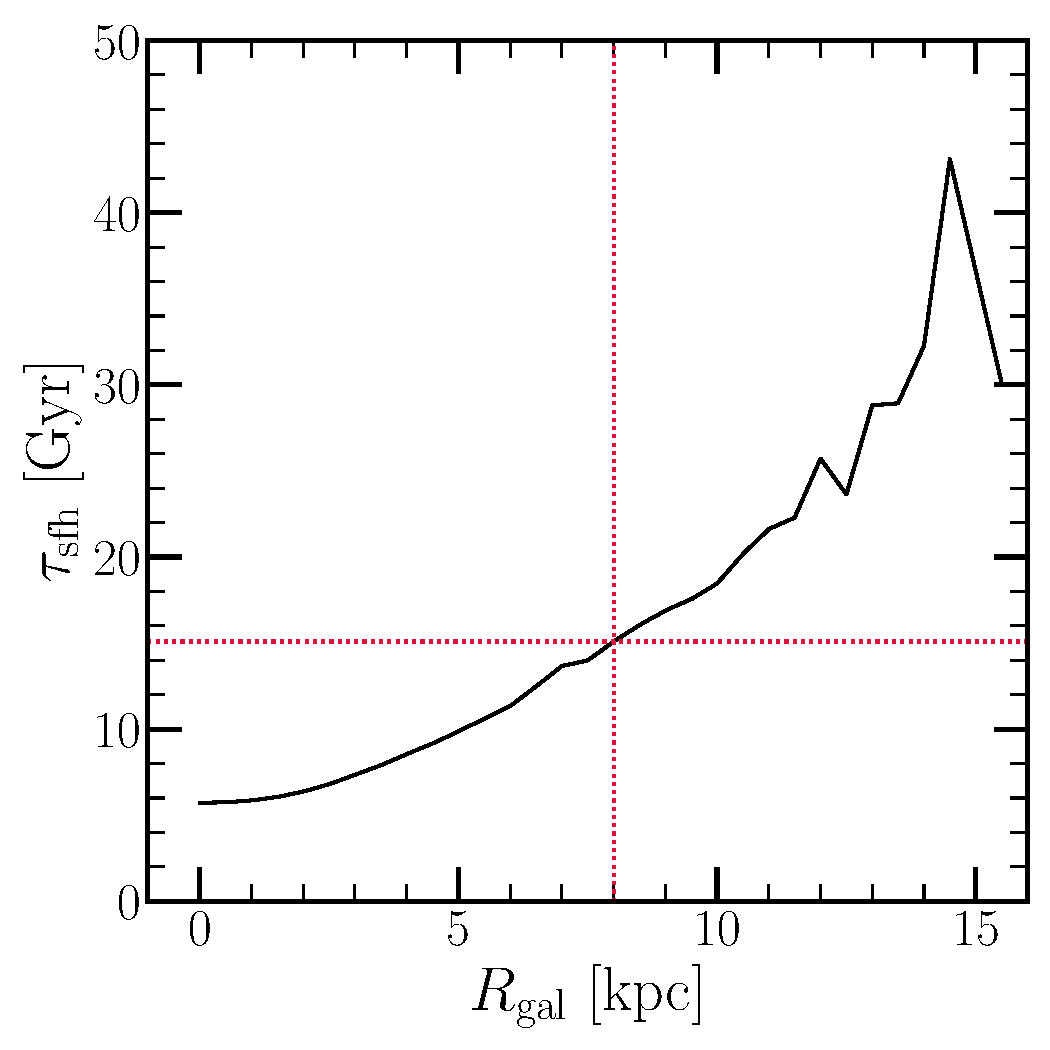
\includegraphics[scale = 0.5]{tau_sfh.pdf} 
\caption{The e-folding timescale of the SFH as a function of Galactocentric 
radius adopted in this work, as reported by Sanchez (2020) for their 
M$_\star$ = $10^{10.5}$ M$_\odot$ - $10^{11.0}$ M$_\odot$ mass bin. The 
horizontal and vertical red dotted lines highlight $\tau_\text{sfh} \approx$ 
15 Gyr at an assumed orbital radius of the sun of R$_\odot$ = 8 kpc. }
\end{figure*} 

\begin{figure*} 
\centering 
\includegraphics[scale = 0.32]{evol/2Gyr_timedep/diffusion.pdf} 
\caption{The surface densities of star formation $\dot{\Sigma}_\star$ (top 
row), infall $\dot{\Sigma}_\text{in}$ (middle row), and gas $\Sigma_\text{gas}$ 
(bottom row) as functions of simulation time in Gyr for our four fiducial 
models - Constant SFR (far left), inside-out (left-middle), late-burst 
(right-middle), and outer-burst (far right). Curves are shown for the annuli 
whose inner radius is 3 kpc (grey), 5 kpc (black), 7 kpc (red), 9 kpc (yellow), 
11 kpc (green), 13 kpc (blue), and 15 kpc (purple). }
\end{figure*} 

\begin{figure*} 
\centering 
\includegraphics[scale = 0.32]{sfe/2Gyr_timedep/diffusion.pdf} 
\caption{The star formation efficiency (SFE) timescale $\tau_\star$ in Gyr 
as a function of Galactocentric radius at simulation times of 2 Gyr (red), 
4 Gyr (yellow), 6 Gyr (green), 8 Gyr (blue), 10 Gyr (purple), and 12.8 Gyr 
(black) for our four fiducial models - Constant SFR (far left), inside-out 
(left-middle), late-burst (right-middle), and outer-burst (far right). }
\end{figure*} 

\begin{figure*} 
\centering 
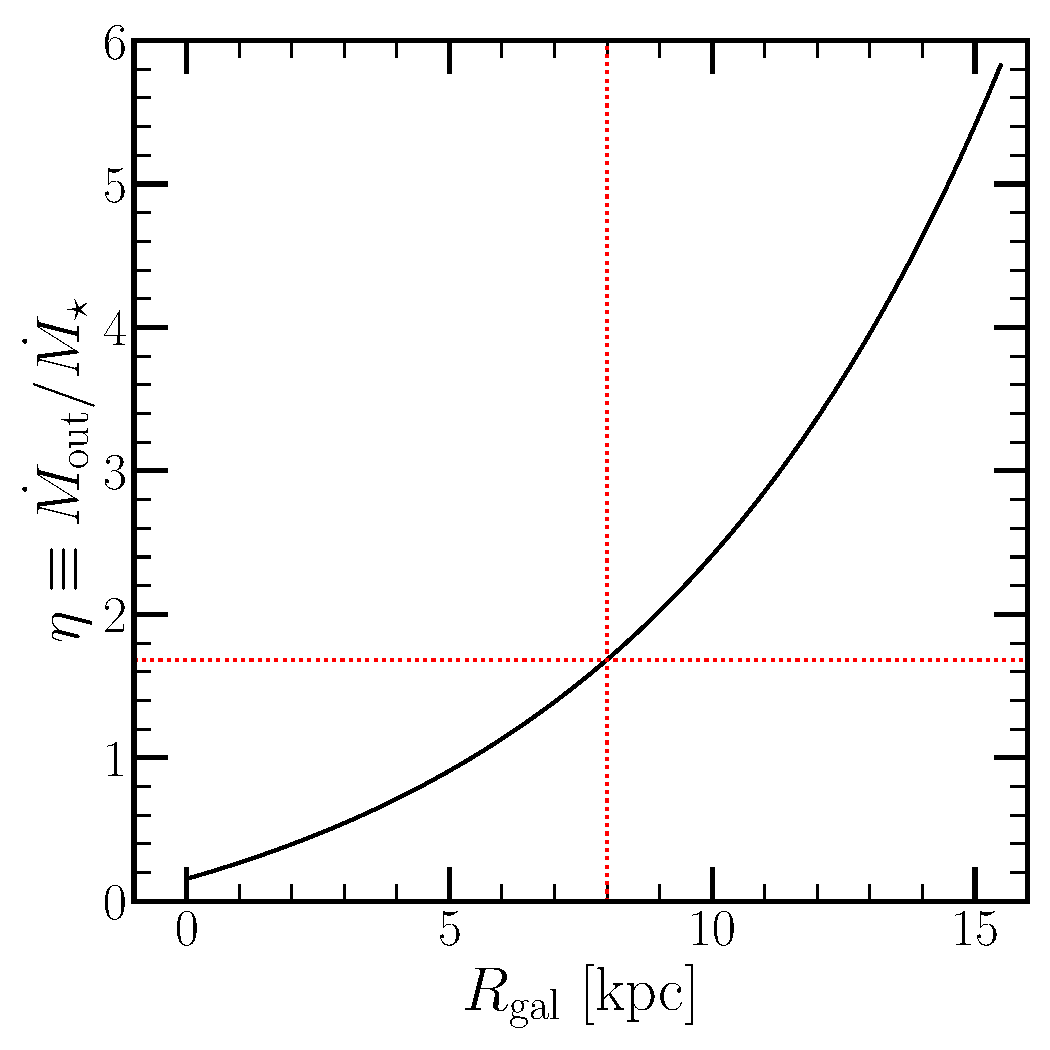
\includegraphics[scale = 0.5]{eta.pdf} 
\caption{Our implemented scaling of the mass loading factor $\eta$ with 
Galactocentric radius (black) as defined by equation X. The horizontal and 
vertical red dashed lines denote the value of $\eta\approx$ 1.7 at an assumed 
orbital radius of the sun of R$_\odot$ = 8 kpc. }
\end{figure*}

\begin{figure*} 
\centering 
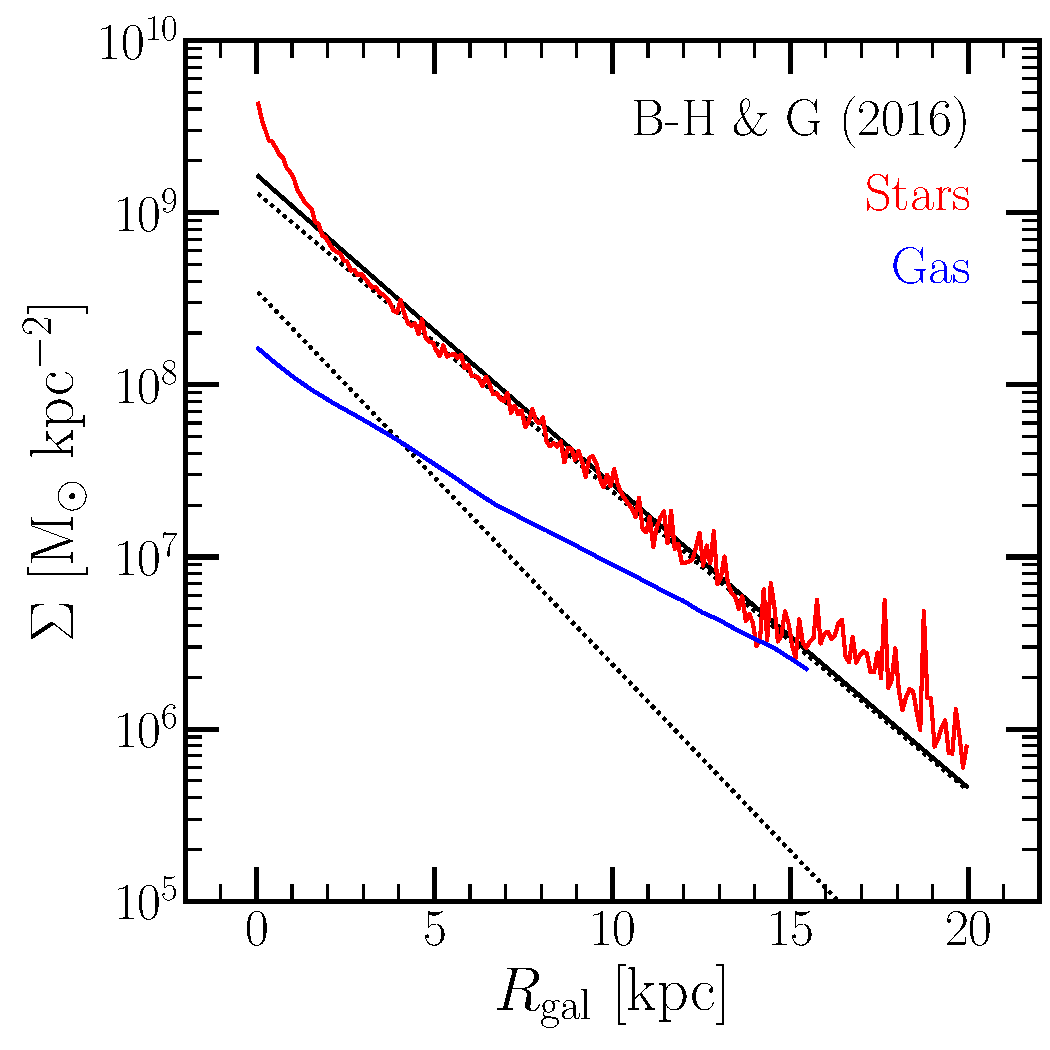
\includegraphics[scale = 0.5]{surface_density_gradient_timedep.pdf} 
\caption{The surface density of gas (blue) and stars (red) as predicted by 
our inside-out evolutionary model with diffusion migration and 
$\tau_\star^\text{mol} = (\text{2 Gyr})(t/t_0)^{1/2}$. For comparison, we 
plot the surface density gradient of the Milky Way thin and thick disks as 
reported by Bland-Hawthorn \& Gerhard (2016) in a black solid line. Black 
dotted lines show the individual thin and thick disk components. }
\end{figure*} 

\begin{figure*} 
\centering 
\includegraphics[scale = 0.32]{metallicity_gradient/2Gyr_timedep/diffusion.pdf} 
\caption{Radial abundance gradients in [O/H] (top, red), [Fe/H] (top, blue), 
and [O/Fe] (bottom) for our four fiducial models - Constant SFR (far left), 
inside-out (left-middle), late-burst (right-middle), and outer-burst 
(far right). We plot the gas-phase abundance at the present day as a function 
of Galactocentric radius in solid lines. Stars denote the mode of the stellar 
MDF of the 100-pc width annulus at a given radius, with shaded regions marking 
the 16th and 84th percentiles thereof. Black lines in the top panels denote 
our target [$\alpha$/H] gradient of mode([$\alpha$/H]) = +0.3 at 
$R_\text{gal}$ = 4 kpc with a slope of -0.06 kpc$^{-1}$. }
\label{fig:metallicity_gradient} 
\end{figure*} 

\begin{figure*} 
\centering 
\includegraphics[scale = 0.45]{tracks/diffusion_2Gyr_timedep.pdf} 
\caption{\textbf{Left}: Evolutionary tracks for the gas phase in the 
[O/Fe]-[Fe/H] plane for models with 
$\tau_\star^\text{mol} = (\text{2 Gyr})(t/t_0)^{1/2}$, our inside-out SFH, and 
either post-processing (dotted lines) or diffusion (solid lines) migration 
models. We plot tracks for seven annuli, color-coded according to their 
Galactocentric radius and denoted by the legend in the lower-left. We mark 
simulation times of 2, 4, 6, 8, 10, and 12.7 Gyr in X's for the diffusion 
model and points for the post-processing model. 
\textbf{Right}: The proxy for the SN Ia rate defined in equation X as a 
function of simulation time for the same annuli as in the left-hand panel. 
We multiply rates at each radii here by various prefactors in the interest of 
clarity. } 
\label{fig:tracks_diffusion} 
\end{figure*} 

\begin{figure*} 
\centering 
\includegraphics[scale = 0.5]{age_ofe/2Gyr_timedep/Rgal_7_9/insideout.pdf} 
\caption{
A comparison of the predicted age-[O/Fe] relation for the solar annulus 
($R_\text{gal}$ = 7 - 9 kpc and $\left|z\right|\leq$ 0.5 kpc) between the 
post-processing (upper left), diffusion (upper right), sudden (lower left), 
and linear (lower right) migration models, assuming our inside-out SFH and 
$\tau_\star^\text{mol} = (\text{2 Gyr})(t/t_0)^{1/2}$. Red triangles and error 
bars denote the observed mean age and dispersion thereof in bins of [O/Fe] as 
reported by Feuillet et al. (2019); here we include only the bins containing 
at least 15 stars. Black squares denote the mass-weighted median age in 
0.02-dex bins in [O/Fe], with error bars denoting the 16th and 84th 
percentiles of the mass-weighted age distribution in those bins. Points in the 
background denote each individual stellar population from the simulation with 
a final position in the solar annulus, color-coded according to their 
Galactocentric radius of birth. 
}
\label{fig:age_ofe_migration_comp}
\end{figure*} 

\begin{figure*} 
\centering 
\includegraphics[scale = 0.5]{age_ofe/2Gyr_timedep/Rgal_7_9/diffusion.pdf} 
\caption{
The same as Fig.~\ref{fig:age_ofe_migration_comp}, instead comparing the 
impact of our constant (upper left), inside-out (upper right), late-burst 
(lower left), and outer-burst (lower right) SFHs, assuming diffusion migration 
and $\tau_\star^\text{mol} = (\text{2 Gyr})(t/t_0)^{1/2}$. 
}
\label{fig:age_ofe_sfh_comp} 
\end{figure*} 

\begin{figure*} 
\centering 
\includegraphics[scale = 0.32]{amr/2Gyr_timedep/diffusion/insideout_O_Fe.pdf} 
\caption{The age-[O/Fe] relation in different galactic regions predicted by 
our inside-out evolutionary model with 
$\tau_\star^\text{mol} = (\text{2 Gyr})(t/t_0)^{1/2}$ and diffusion migration. 
Bins in Galactocentric radius are shown in columns, and labeled at the top. 
Bins in the height $\left|z\right|$ above/below the disk midplane are shown in 
rows, noted in the left-hand column. Red triangles and error bars denote the 
observed mean age and dispersion thereof in bins of [O/Fe] as reported by 
Feuillet et al. (2019); here we include only the bins containing at least 
15 stars. Black squares denote the mass-weighted median age in 0.02-dex bins 
in [O/Fe], with error bars denoting the 16th and 84th percentiles of the 
mass-weighted age distribution in those bins. Points in the background denote 
each individual stellar population from the simulation with a final position 
in that Galactic region, color-coded according to their Galactocentric radius 
of birth. 
} 
\label{fig:galactic_regions_ofe} 
\end{figure*} 

\begin{figure*} 
\centering 
\includegraphics[scale = 0.32]{amr/2Gyr_timedep/diffusion_O.pdf} 
\caption{
The age-[O/H] relation predicted by our constant (top), inside-out (top 
middle), late-burst (bottom middle), and outer-burst (bottom) SFHs for 
$R_\text{gal}$ = 5 - 7 kpc (left), 7 - 9 kpc (left middle), 9 - 11 kpc (right 
middle), and 11 - 13 kpc (right). Each panel plots only the 
$\left|z\right|\leq$ 0.5 kpc population. Background points, red triangles with 
error bars, and black squares with error bars are as in 
Fig.~\ref{fig:galactic_regions_ofe}, but with our binned, simulated relation 
quantified in 0.05-dex bins in [O/H]. 
}
\label{fig:disk_comp_o} 
\end{figure*} 

\begin{figure*} 
\centering 
\includegraphics[scale = 0.32]{amr/2Gyr_timedep/diffusion_Fe.pdf} 
\caption{The same as Fig.~\ref{fig:disk_comp_o}, but for the age-[Fe/H] 
relation.} 
\label{fig:disk_comp_fe} 
\end{figure*} 

\begin{figure*} 
\centering 
\includegraphics[scale = 0.32]{amr/2Gyr_timedep/diffusion/outerburst_O.pdf} 
\caption{The same as Fig.~\ref{fig:galactic_regions_ofe}, but for the age-[O/H] 
relation, the outer-burst rather than inside-out SFH, and with our binned, 
simulated relation quantified in 0.05-dex bins in [O/H].} 
\label{fig:galactic_regions_o}
\end{figure*} 

\begin{figure*} 
\centering 
\includegraphics[scale = 0.32]{amr/2Gyr_timedep/diffusion/outerburst_Fe.pdf} 
\caption{The same as Fig.~\ref{fig:galactic_regions_ofe}, but for the 
age-[Fe/H] relation, the outer-burst rather than inside-out SFH, and with our 
binned, simulated relation quantified in 0.05-dex bin in [Fe/H].}
\label{fig:galactic_regions_fe}
\end{figure*} 

\begin{figure*} 
\centering 
\includegraphics[scale = 0.4]{mdf_3panel/2Gyr_timedep/diffusion/insideout.pdf} 
\caption{Metallicity distribution functions (MDFs) in [Fe/H] for our 
inside-out SFH with $\tau_\star^\text{mol} = (\text{2 Gyr})(t/t_0)^{1/2}$ and 
diffusion migration. Distributions are shown in bins of present-day 
Galactocentric radius noted in the legend in the top panel, with each panel 
showing distributions in bins of $\left|z\right|$ noted at the top-center of 
each panel.}
\label{fig:mdf_3panel_insideout} 
\end{figure*} 

\begin{figure*} 
\centering 
\includegraphics[scale = 0.4]{mdf_3panel/2Gyr_timedep/diffusion/lateburst.pdf} 
\caption{Same Fig.~\ref{fig:mdf_3panel_insideout}, but for our late-burst SFH.}
\end{figure*} 

\end{document}
